\documentclass[epsf]{article}
\usepackage{amsmath,amsthm,amsfonts,latexsym,amscd, framed}
\usepackage{graphicx}

\textwidth=6.0truein\hoffset=-.5truein
\textheight=8.5truein\voffset=-.5truein

\begin{document}
%\maketitle
\newcommand{\R}{\mathbb{R}}
\newcommand{\noi}{\noindent}
\newcommand{\bs}{\bigskip}

%%%%

\vspace{-0.5 in}
\noi NAME(S): \line(1,0){130} \hspace{.2in}TA (circle one): Elizabeth \ \ \ Christian 
\vskip .2 in
\hspace{.44 in} \line(1,0){130} \hspace{.2in}SECTION (circle one): 8AM \ 12PM\ 4PM \ 5PM 
\vskip 1mm
\hspace{3.9 in} 6PM\ \ 7PM


\begin{center}
{\Large Project \#4: Phase Portraits for Linear DE Systems\\
\vskip 2mm
Solutions Page}

\vskip 4mm
Feedback\footnote{Please see DP Evaluation Rubric handout, available on GauchoSpace, for more information on how DP solutions are evaluated.}
\vskip 2mm
\begin{tabular}{| l | c |}
\hline
 & \\
quality of mathematical ideas (7 pts) &  \hspace{2 cm}   \\
 & \\
\hline
 & \\
clarity of communication (3 pts) & \\
 & \\
\hline
\end{tabular}
\end{center}



\vskip 2mm
Please write your group or individual solution on this page.  Staple any additional work for your solutions on the back of this page to turn in during section on Wednesday, December 10th.  If you cannot attend section, get your solutions to your TAs mailbox in SH 6623 by 4:00pm the day your section meets.\\

\noi{\bf Problem 1} Consider the system
$$\vec{\bf x}' = \begin{bmatrix}\ \ 3 & -2 \cr -1 &\ \ 2 \end{bmatrix}\vec{\bf x}.$$
The matrix of the system has eigenvalues/vectors:
$$ \lambda_1 = 1, \ \ \vec{\bf v}_1 = \begin{bmatrix}1\cr 1 \end{bmatrix} \ \ \text{and} \ \ \lambda_2 = 4,\ \ \vec{\bf v}_2= \begin{bmatrix}-2\cr \ \ 1 \end{bmatrix}$$
\begin{itemize}
\item[(a)] Write down the general solution for the system.
\vskip 1  in
\item[(b)] Is the equilibrium solution $\vec{\bf 0}$ a source, sink or saddle? Explain.\footnote{Please provide all of your explanations in complete sentences.}
\newpage

\item[(c)] Which eigenvector corresponds to the ``fast'' direction and which corresponds to the ``slow'' direction?  Explain how you know and how this will affect solutions trajectories as they move away from the origin.
\vskip 1.5 in
\item[(d)] Which of the phase portraits corresponds to this system?
\end{itemize}

\vskip 1in

\noi{\bf Problem 2} Consider the system
$$\vec{\bf x}' = \begin{bmatrix} 1 & -1 \cr 5 & -1 \end{bmatrix}\vec{\bf x}.$$
The matrix of the system has eigenvalues/vectors:
$$ \lambda_1 = 2i, \ \ \vec{\bf v}_1 = \begin{bmatrix}1\cr 1 \end{bmatrix} + i\begin{bmatrix}0 \cr 2 \end{bmatrix}\ \ \text{and} \ \ \lambda_2 = -2i,\ \ \vec{\bf v}_2= \begin{bmatrix}1\cr 1 \end{bmatrix} - i\begin{bmatrix}0 \cr 2 \end{bmatrix}$$

\begin{itemize}
\item[(a)] Write down the general solution for the system.
\vskip 1in
\item[(b)] Are solution trajectories in the phase plane oscillating?  Are they periodic? Explain how you can tell.
\newpage

\item[(c)] Since the eigenvalues are complex, there should be some sort of rotation in the phase plane.  Will this rotation be clockwise or counterclockwise?  Explain how you can tell.
\vskip 2 in
\item[(d)] Which of the phase portraits corresponds to this system?
\end{itemize}

\newpage

Use the following phase portraits to answer part (d) of problems 1 and 2. \\


\begin{center}
A 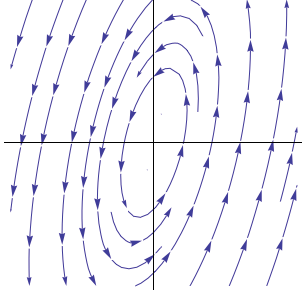
\includegraphics[width=40mm]{center1.png}\hspace{0.6 cm}B 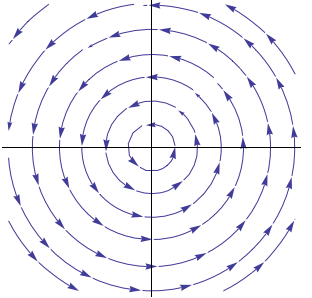
\includegraphics[width=40mm]{center2.png}\hspace{0.6cm}C 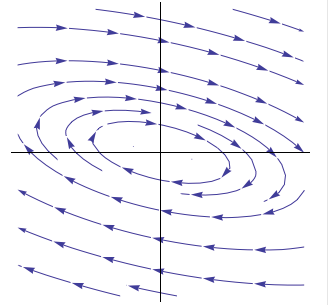
\includegraphics[width=40mm]{center3.png}\\

\vskip 1cm
D 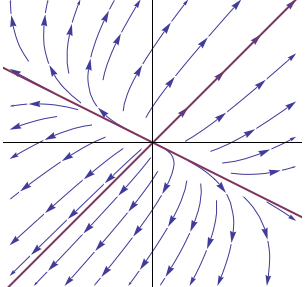
\includegraphics[width=40mm]{source1.png}\hspace{0.6 cm} E 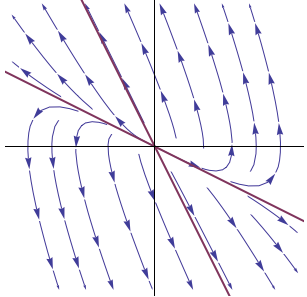
\includegraphics[width=40mm]{source2.png}\hspace{0.6 cm} F 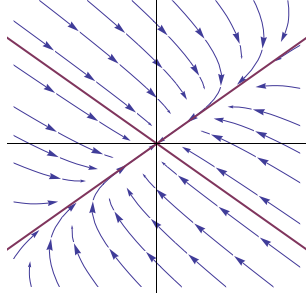
\includegraphics[width=40mm]{sink.png}\\
\vskip 1cm
G 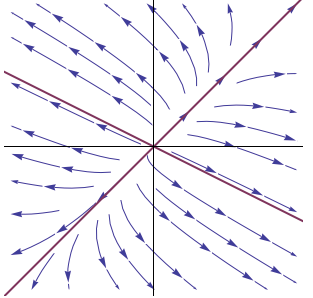
\includegraphics[width=40mm]{source4.png}\hspace{0.6 cm} H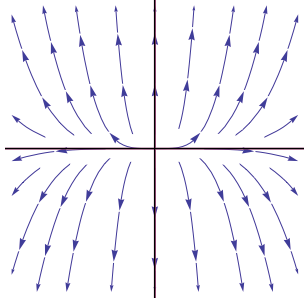
\includegraphics[width=40mm]{source3.png}\hspace{0.6 cm} I 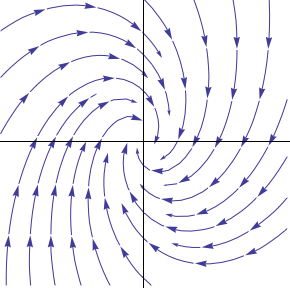
\includegraphics[width=40mm]{stable_spiral.png}\\
\vskip 1cm
J 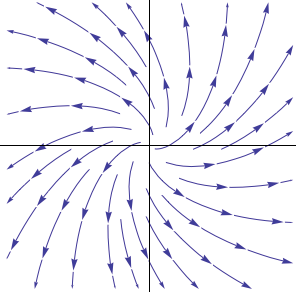
\includegraphics[width=40mm]{spiral_source.png}\hspace{0.6 cm} K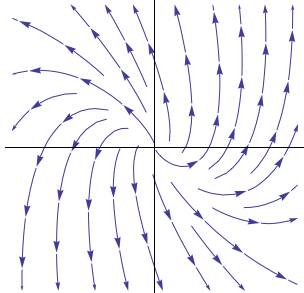
\includegraphics[width=40mm]{spiral_source2.png}\hspace{0.6 cm} L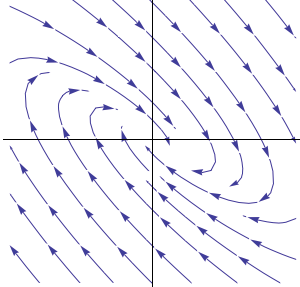
\includegraphics[width=40mm]{stable_spiral2.png}\\
\end{center}

\end{document}
%%%%%%%%%%%%%%%%%%%%%%%%%%%%%%%%%%}

\begin{enumerate}
\item Next we consider a more challenging system
\begin{equation}
\label{N2}
\vec{x}' =\begin{bmatrix}1 & 1 \cr 4 & 1 \end{bmatrix}\vec{x} + \begin{bmatrix} 2t \cr 0 \end{bmatrix}.
\end{equation}

\vskip 2mm

\noindent (a) By writing (\ref{N2}) in the right coordinates, we \textit{decouple} the system and can easily solve it.  Let $\mathcal{B} = \{\vec{v}_1, \vec{v}_2 \}$, where 
$$\vec{v}_1 := \begin{bmatrix}1 \cr 2 \end{bmatrix} \text{ and } \vec{v}_2 := \begin{bmatrix}\ \ 1 \cr -2 \end{bmatrix}$$ 
are linearly independent eigenvectors of the matrix $A = \begin{bmatrix}1 & 1 \cr 4 & 1 \end{bmatrix}$.  Let $\vec{w}:= (\vec{x})_{\mathcal{B}}$ and write down the system for $\vec{w}$ - you should get a (very familiar) decoupled nonhomogeneous system.  What is $\vec{w}(t)$?

\vskip 2mm
\noindent (b) Use a change-of-coordinates to compute $\vec{x}(t)$.

\vskip 2mm
\noindent (c) Since this is one of the first nonhomogeneous system you've solved, I strongly suggest that you verify that your solution $\vec{x}$ satisfies the original system (\ref{N2}).

\vskip 2mm
\noindent (d) Describe the solution space for (\ref{N2}).\\

\item Solve the following nonhomogeneous systems by decoupling them.
\vskip 2mm
\noi (a) $$\vec{\bf x}' = \begin{bmatrix} 2 & -1 \cr 3 & -2  \end{bmatrix} \vec{\bf x} + \begin{bmatrix}e^t \cr t \end{bmatrix}.$$
\vskip 2mm

\noi(b) For this one, you will have to work with complex coordinates. $$\vec{\bf x}' = \begin{bmatrix} 2 & -5 \cr 1 & -2  \end{bmatrix} \vec{\bf x} + \begin{bmatrix}-\cos t \cr \sin t\end{bmatrix}.$$\\

\item For the homogeneous system
\begin{equation}
\label{J}
\vec{x}' = \begin{bmatrix}\ \ 2 & 1 \cr -1 & 4 \end{bmatrix}\vec{x},
\end{equation}  
decoupling hits a snag: The matrix $B := \begin{bmatrix}\ \ 2 & 1 \cr -1 & 4 \end{bmatrix}$ does not have two linearly independent eigenvalues, so $B$ cannot be diagonalized (and the system cannot be solve our usual way).  However, the matrix can be put in the \textit{Jordan form}:
\begin{equation*}
J = \begin{bmatrix}\lambda & 1\cr 0 & \lambda \end{bmatrix}
\end{equation*} 
where $\lambda$ is the eigenvalue for $B$.  To do this we must change the coordinates for $B$ to the basis $\mathcal{B} = \{\vec{v}, \vec{u} \}$ where $\vec{v}$ is an eigenvector associated with the eigenvalue $\lambda$ and $\vec{u}$ is a solution to the equation $(A - \lambda I)\vec{u} = \vec{v}$.  We call   $\vec{u}$ a \textit{generalized eigenvector} of $B$.
\vskip 2mm
\noindent (a) Compute $\lambda$, $\vec{v}$ and $\vec{u}$ and verify that $[B]_{\mathcal{B}} = J$.

\vskip 2mm
\noindent (b) Show how you can use a modified decoupling method to solve the system (\ref{J}).

\vskip 2mm
\noindent (c) It's a good idea to double check your solution to (\ref{J}) now.

\end{enumerate}
\end{document}
